\chapter{Gestaltung der Arbeit}
\section{Zielgruppe}

Die Zielgruppe einer Arbeit sind in der Regel Studierende im gleichen Studienverlauf wie Sie.
Inhalte aus dem Pflichtstudium oder vorausgesetzten Modulen können Sie daher
als bekannt voraussetzen, und für diese sind auch meist keine Quellenangaben
notwendig (bspw.{} QuickSort können Sie ohne Quellenangabe nennen).
Bei einer Seminararbeit können Sie auch Grundlagen aus dem Rahmenthema als bekannt voraussetzen.
Bei Abschlussarbeiten können Sie auch Vertiefungsmodule der Arbeitsgruppe als Grundwissen ansehen,
dass sie nicht wiederholen müssen.

Versuchen Sie ihre Arbeit so zu erstellen, dass sie einen \emph{Mehrwert} für diese Zielgruppe
liefert, und für diese \emph{gut verständlich} ist. Die Betreuer*innen hingegen werden in der Regel die
Originalquellen kennen oder bevorzugen. Um den Rückgriff auf diese zu vereinfachen, sollten
sie wie üblich zitiert sein.

\section{Sprache}
Laden Sie die passenden Sprachpakete mit \texttt{babel}. Das letztgenannte Sprachpaket legt dabei die Hauptsprache der Arbeit fest.
Mit der korrekten Sprache werden bestimmte Überschriften (bzw.{} \enquote{Literaturverzeichnis}) richtig erzeugt,
der Anführungszeichenstil angepasst, und insbesondere die \emph{korrekte Silbentrennung} aktiviert.

\begin{otherlanguage}{english}
You can temporarily switch the language to obtain correct hyphenation in other
languages. Simply use an \texttt{otherlanguage} environment.
This also affects quotes and citations, e.g., \enquote{\textcite{Deininger2017}} is now quoted differently.
\end{otherlanguage}

Es mag ihnen auf den ersten Blick einfacher \emph{erscheinen}, auf Deutsch zu schreiben.
Da aber ein Großteil der Quellen und Fachbegriffe auf Englisch ist, kommt dann schnell ein ziemlicher Kauderwelsch heraus,
auch bekannt als \enquote{Denglisch}. Des Weiteren neigen die meisten auf
Deutsch zu \enquote{Schachtelsätzen}, worunter die Lesbarkeit stark leidet,
während es auf Englisch den meisten leichter fällt, einen einfacheren Satzbau
zu verwenden.
Viele der Schwierigkeiten mit geschlechtergerechter Sprache entfallen
ebenfalls, wenn Sie auf Englisch schreiben, insbesondere wenn man auf den
Plural (they statt he/she) ausweichen kann.
Eine sogenannte \enquote{Generalklausel} erfüllt nicht das Ziel,
sprachinduzierte Stereotype aufzulösen.
Für Sie besteht aber aktuell wohl keine Verpflichtung zum Gendern, lediglich
eine Empfehlung, und daher wird dies nicht bei der Benotung berücksichtigt.%
\footnote{Siehe: \url{https://gleichstellung.tu-dortmund.de/themen/geschlechtergerechte-sprache/}}
Es empfiehlt sich dennoch, dies zu üben.

Wenn Sie später einmal eine wissenschaftliche Arbeit international
veröffentlichen wollen -- beispielsweise Teile ihrer Masterarbeit --
wird dies auf Englisch erfolgen müssen, damit sie auch gelesen wird.
Daher ist es eine gute Übung, bereits bei Seminar- und Bachelorarbeiten auf Englisch zu schreiben.
Zudem gibt es für Englisch meist die besseren Werkzeuge bspw.{} zur Grammatikprüfung.

Auf jeden Fall sollten Sie in ihrem Editor eine \emph{Rechtschreibprüfung} installieren und einsetzen!
Es empfiehlt sich auch, schwierige Sätze mit einer Grammatikprüfung zu validieren.
Auch Verwandte, Bekannte und Mitstudierende können helfen, Fehler zu finden.
Rechtschreib- und Grammatikfehler hinterlassen immer einen schlechten ersten Eindruck.

\section{\LaTeX{}-Vorlage}

%In diesem Seminar wird erwartet, dass die zur Verfügung gestellte \LaTeX{}-Vorlage verwendet wird.
Mit Hinblick auf die Anforderungen der Disziplin, insbesondere Formelsatz
und Quellenangaben, ist \LaTeX{} derzeit Mittel der Wahl.
Auch wenn manche Studierende eine Konvertierung von Markdown nach \LaTeX{} bevorzugen,
so gewinnt man damit nur sehr wenig -- die in Markdown möglichen Formatierungen sind
auch in \LaTeX{} kein großer Mehraufwand, und der Umweg über Markdown bietet
hier nahezu keine Vorteile.

\section{Literatur}

Legen Sie bereits \textit{beim Lesen} eine Literaturdatenbank an,
sinnvollerweise im Bibtex-Format. Saubere Bibtex-Einträge finden
Sie für einen Großteil der Informatik-Literatur auf \url{https://dblp.org/}.
Das Open-Source Werkzeug JabRef (\url{https://jabref.org/}) kann bequem aus DBLP importieren.
Nichts ist ärgerlicher, als wenn Sie eine verwendete Quelle selbst nicht mehr wiederfinden!

\emph{Kopieren Sie nicht aus anderen Werken.} Wörtliche Zitate sind in der Informatik
eher unüblich. Wenn Sie wirklich etwas aus einer Quelle übernehmen (bspw.{} eine Grafik),
fügen Sie \textbf{immer als erstes die Quellenangabe} ein, dann vergessen Sie das nicht.
Wörtliche Übernahmen setzen Sie \emph{sofort in Anführungszeichen}.
Auch ein automatisches Paraphrasieren ist \emph{nicht empfehlenswert}.
Sie sollen zeigen, dass Sie die Quelle verstanden haben, nicht dass Sie
Strg+C kennen. Plagiate sind nicht akzeptabel!
Geben Sie dazu die Inhalte mit ihren eigenen Worten wieder -- dann kann man beim
genauen Lesen bspw.{} nachvollziehen, warum Sie zu einem anderen Ergebnis gekommen sind.

\texttt{biblatex} (mit \texttt{biber}) ist eine modernere und konfigurierbare Alternative zu dem
klassischen \texttt{bibtex}, das Sie in vielen Anleitungen noch finden.
Deswegen setzen wir in dieser Vorlage auf biblatex.

Kontrollieren Sie das Literaturverzeichnis! Hier finden sich oft peinliche Fehler.
So war in einem Literaturverzeichnis durch einen nicht korrigierten Parsing-Fehler
von Google Scholar die fehlerhafte Autorenangabe
\enquote{Petra \mbox{\emph{Stein-Sven}} Vollnhals} statt der korrekten Angabe
\enquote{Petra Stein und Sven Vollnhals}.

Mit den Kommandos \texttt{\textbackslash{}textcite\{\}} und 
\texttt{\textbackslash{}parencite\{\}} können Sie Quellen zitieren.
Dabei ist bei der Verwendung als Subjekt in einem Satz die Verwendung von
Beispiel: \textcite{Deininger2017} bzw.{} am Ende eines Satzes~\parencite{Voss2022}.

Das Kommando \texttt{\textbackslash{}fullcite\{\}} erlaubt auch eine komplette
Angabe im Fließtext (siehe oben), was sich aber nur für herausragende Quellen
anbietet (bspw.{} die Hauptquelle einer Seminar- oder Bachelorarbeit).

Quellenangaben mit \texttt{\textbackslash{}textcite\{\}} kommen an die richtige
Stelle im Satzbau, oftmals ist dies das Subjekt am Anfang des Satzes.
Ein Satz sollte ohne die Klammern immer noch Sinn ergeben, daher sollte
\texttt{\textbackslash{}parencite\{\}} nur verwendet werden, wenn es grammatikalisch nicht mitgelesen werden muss.
Quellenangaben die sich nur auf einen Begriff beziehen direkt hinter diesen.
Beziehen sie sich jedoch auf den ganzen Satz, so kommen sie in der Regel vor das Satzzeichen.
Manche Autor*innen nutzen Quellenangaben nach dem letzten Satzzeichen, wenn sie sich auf den gesamten Absatz beziehen.

Internetquellen sind mit Vorsicht zu handhaben, denn die Webseiten können sich jederzeit ändern.
Deswegen müssen Sie das Zugriffsdatum mit angeben. Idealerweise sichern sie eine Kopie der Seite,
entweder bei ihren Unterlagen oder mit einem Archivdienst wie \url{https://web.archive.org/} oder \url{https://archive.is/}.
Zudem lassen sich Autor*innen nicht immer klar identifizieren. Sind Autor*innen genannt, beispielsweise bei einem Zeitungsartikel,
dann \emph{müssen} Sie diesen aber auch in der Quellenangabe nennen.
Wikipedia \emph{hat} ein Zitationswerkzeug, mit dem Sie einen Link zu einer spezifischen Version der Seite erstellen können,
kann aber dennoch Fehler in den BibTeX-Einträgen enthalten.

\section{Aufzählungen}

Da dies keine PowerPoint-Präsentation ist, werden sie selten Aufzählungen benötigen.
\begin{itemize}
\item einfach mehrere \texttt{\textbackslash{}item}s erstellen
\item auch nicht komplizierter als Markdown...
\end{itemize}

\noindent % keine ganze Zeile
Natürlich gibt auch nummerierte Aufzählungen.
\begin{enumerate}
\item Eins
\item Zwei
\end{enumerate}

Aus Platzgründen ist es oftmals aber geschickt, Aufzählungen im Text eingebettet zu verwenden: \texttt{(1)\textasciitilde Eins, (2)\textasciitilde Zwei}.

\section{Schriftsatz und Typografie}

Weder im Deutschen noch im Englischen macht man Leerzeichen von Satzzeichen.
Nach einem Satzzeichen wird ein größerer Abstand verwendet, dies macht aber \LaTeX{}
automatisch. Um das zu verhindern -- bspw.{} bei Abkürzungen -- können Sie entweder
\texttt{.\{\}} verwenden, oder ein geschütztes Leerzeichen \texttt{\textasciitilde}.
Geschützte Leerzeichen sind des weiteren hilfreich (1)~vor Quellenangaben, d.h., \texttt{\textasciitilde\textbackslash{}parencite\{\}},
(2)~bei um einen Zeilenumbruch innerhalb von logischen Einheiten zu verhindern
(bspw.{} \texttt{in 3\textasciitilde{}Dimensionen.}), oder um unschöne Umbrüche am Ende eines Satzes
oder in einer Aufzählung zu verhindern (bspw.{} \texttt{(1)~vor Quellenangaben}).
Leere Klammern~\texttt{\{\}} sind auch bei Makros oft hilfreich um Ambiguitäten zu vermeiden.
Möchten Sie den Zeilenumbruch bspw.{} in einem Algorithmennamen vermeiden, so
können Sie mit \texttt{\textbackslash{}mbox\{QuickSort\}} einen Umbruch verhindern.

Unterschieden wird zwischen einem Bindestrich (data-set), der mathematischen Operation~\mbox{($a-b$)},
einem Gedankenstrich~\mbox{(--)}, und einem langen Strich~\mbox{(---)}.
Um Text zu betonen nutzen Sie vorwiegend \texttt{\textbackslash{}emph\{\}} statt \textbf{Fettdruck},
während \underline{Unterstriche} als veraltet gelten.
Mit \texttt{\textbackslash{}enquote\{\}} können Sie korrekte Anführungszeichen setzen,
\enquote{auch wenn diese \enquote{geschachtelt} sind.}
Apostrophen sind im Deutschen fast nur als Auslassungszeichen richtig, nicht bei jedem Genitiv oder gar Plural.

\section{Tabellen}

In Tabelle~\ref{tab:Beispiele} sehen Sie ein Beispiel für eine Tabelle als Fließobjekt auf der Seite.
Aufgrund der Plazierungslogik von \LaTeX{} ist es meist geschickt, die Tabelle am Anfang des
Abschnitts in dem sie verwendet werden soll einzufügen.

\begin{table}[h!]
\caption{Tabellen haben ihre Beschreibung in der Regel oben (Bilder unten), und es werden nur
sparsam Linien verwendet.}
\label{tab:Beispiele}
\begin{tabular*}{\linewidth}{@{}llr@{.}l@{~}l@{}}
\toprule
Links & Rechts & \multicolumn{3}{c}{ausgerichtete Zahlen} \\
\midrule
links & rechts & 123 & 45 & ms \\
links & rechts &   3 & 45 & s \\
\bottomrule
\end{tabular*}
\end{table}

Mit den Buchstaben \texttt{bth} können Sie die
Platzierung steuern. Die \enquote{here} (\texttt{h}) Platzierung ist dabei eher ungewöhnlich.
Fließobjekte am Anfang (\texttt{t}) oder Ende (\texttt{b}) einer Seite spart in der Regel Platz
aufgrund der nötigen Abstände vor und nach eines Fließobjektes.
Und gerade bei größeren Tabellen kann eine \enquote{here} Platzierung einen Seitenumbruch nötig machen.
Bei einer echten Verwendung im Text kann es passender sein, nur ein \texttt{tabbing} einzusetzen.
Versehen Sie jede Tabelle mit einem \texttt{\textbackslash{}label\{tab:uniqueid\}},
dann erhalten Sie mit \texttt{Tabelle\textasciitilde{}\textbackslash{}ref\{tab:uniqueid\}}
eine automatische Referenz darauf.

\section{Bilder und Grafiken}

Bilder können in \LaTeX{} mit dem Kommando \texttt{\textbackslash{}includegraphics} eingebunden werden.
Dabei bieten sich für \texttt{pdflatex} die Dateiformate \texttt{.png},
\texttt{.jpg} und \texttt{.pdf} (für Vektorgrafiken) an.
Bilder werden in der Regel als Fließobjekt in einer \texttt{\textbackslash{}figure}-Umgebung
platziert, im Gegensatz zu Tabellen steht hierbei die \texttt{\textbackslash{}caption}
aber unterhalb. Die Verwendung von \texttt{\textbackslash{}label} und \texttt{\textbackslash{}ref} ist analog.

\begin{figure}[bt!h]\centering

\includegraphics[width=.8\textwidth]{bilder/schlechte-qualitaet.png}
\caption{Screenshots sehen eigentlich immer unscharf aus, aber gerade Subpixel-Antialiasing (links) führt zu unschönen Farbschlieren.}
\label{fig:screenshots}
\end{figure}

Achten Sie unbedingt auf eine ausreichende Bildqualität!
Ein Bildschirmfoto sieht oftmals gedruckt auf einmal sehr schlecht aus, insbesondere ein Bildschirmfoto von Text.
Wenn ihr System dabei Subpixel-Antialiasing einsetzt können unerwünschte Farbschlieren entstehen (vgl.{} Abbildung~\ref{fig:screenshots}).
Überlegen Sie, ob sie nicht das gewünschte Material (1)~als Text, (2)~als Vektorgrafik, oder (3)~hochauflösend erstellen können. Bspw.{} können Sie im Browser den Zoom erhöhen bevor Sie einen Screenshot einer Webseite machen.

\begin{figure}[bt!]\centering
\begin{tikzpicture}
\begin{axis}[axis lines=left,xlabel=$x$,ylabel={$f(x)$},ymax=1.8]
\addplot[domain=-1.3:1.3, samples=100, color=blue, very thick]{x^2};
\addlegendentry{$x^2$}
\end{axis}
\end{tikzpicture}
\caption{Diagramm einer Parabel mit \texttt{pgfplots}, wodurch die Schriften und -größen des Dokuments verwendet werden.}
\label{fig:parabel}
\end{figure}

Mit den Paketen \texttt{tikz} und \texttt{pgfplots} lassen sich auch komplexe Grafiken und Diagramme
in \LaTeX{} selbst \enquote{programmieren}.
Abbildung~\ref{fig:parabel} zeigt eine Parabel mit \texttt{pgfplots}, die so erzeugte Grafik ist konsistent mit dem Rest des Dokuments.
Ein wesentlicher Vorteil dabei ist, dass dann die Schriften im Dokument konsistent sind,
und man beispielsweise mathematische Formeln problemlos in Beschriftungen verwenden kann.

Aber auch mit Python's \texttt{matplotlib} kann man gute Qualität erzielen. Man sollte dann die Schriftart, Schriftgröße, und Größe des Bildes passend einstellen, und im PDF-Format ausgeben.
Den Qualitätsunterschied können Sie in Abbildung~\ref{fig:pyplot} sehen. Matplotlib kann auch direkt nach \texttt{.tex} ausgeben, bspw.{} für die \texttt{pgfplots} Bibliothek.

\begin{figure}
\begin{subfigure}{.5\textwidth}\centering
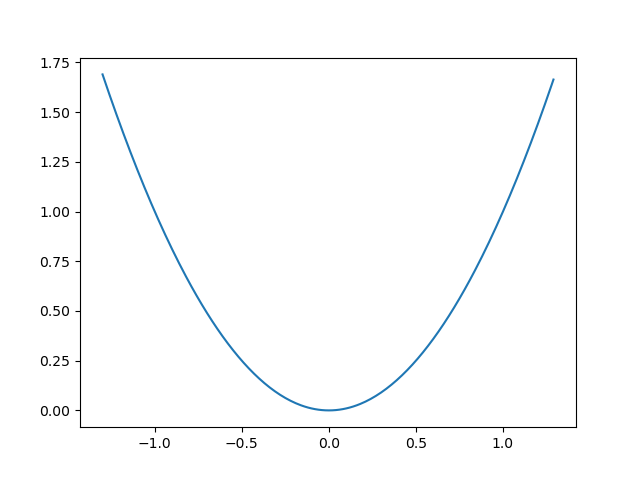
\includegraphics[width=\linewidth]{bilder/pyplot1.png}
\caption{Einfacher Python-Plot, Ergebnis}
\end{subfigure}
\begin{subfigure}{.5\textwidth}\centering
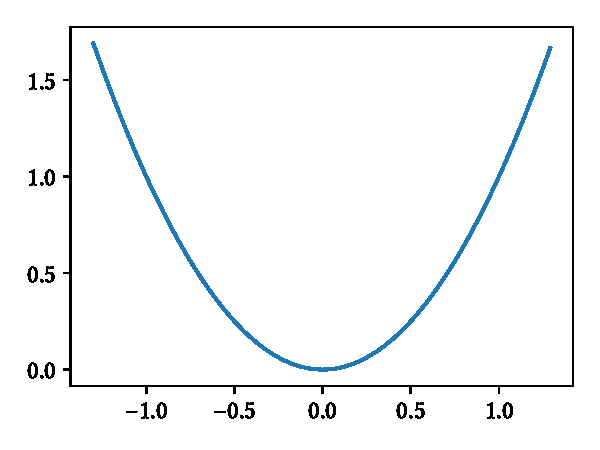
\includegraphics[width=\linewidth]{bilder/pyplot2.pdf}
\caption{PDF Python-Plot, Ergebnis}
\end{subfigure}
\\
% Eigentlich an Dokumentanfang, hier nur im Beispiel inline
% pygmentize -f latex -S friendly > generiert/friendly.tex

\makeatletter
\def\PY@reset{\let\PY@it=\relax \let\PY@bf=\relax%
    \let\PY@ul=\relax \let\PY@tc=\relax%
    \let\PY@bc=\relax \let\PY@ff=\relax}
\def\PY@tok#1{\csname PY@tok@#1\endcsname}
\def\PY@toks#1+{\ifx\relax#1\empty\else%
    \PY@tok{#1}\expandafter\PY@toks\fi}
\def\PY@do#1{\PY@bc{\PY@tc{\PY@ul{%
    \PY@it{\PY@bf{\PY@ff{#1}}}}}}}
\def\PY#1#2{\PY@reset\PY@toks#1+\relax+\PY@do{#2}}

\@namedef{PY@tok@w}{\def\PY@tc##1{\textcolor[rgb]{0.73,0.73,0.73}{##1}}}
\@namedef{PY@tok@c}{\let\PY@it=\textit\def\PY@tc##1{\textcolor[rgb]{0.38,0.63,0.69}{##1}}}
\@namedef{PY@tok@cp}{\def\PY@tc##1{\textcolor[rgb]{0.00,0.44,0.13}{##1}}}
\@namedef{PY@tok@cs}{\def\PY@tc##1{\textcolor[rgb]{0.38,0.63,0.69}{##1}}\def\PY@bc##1{{\setlength{\fboxsep}{0pt}\colorbox[rgb]{1.00,0.94,0.94}{\strut ##1}}}}
\@namedef{PY@tok@k}{\let\PY@bf=\textbf\def\PY@tc##1{\textcolor[rgb]{0.00,0.44,0.13}{##1}}}
\@namedef{PY@tok@kp}{\def\PY@tc##1{\textcolor[rgb]{0.00,0.44,0.13}{##1}}}
\@namedef{PY@tok@kt}{\def\PY@tc##1{\textcolor[rgb]{0.56,0.13,0.00}{##1}}}
\@namedef{PY@tok@o}{\def\PY@tc##1{\textcolor[rgb]{0.40,0.40,0.40}{##1}}}
\@namedef{PY@tok@ow}{\let\PY@bf=\textbf\def\PY@tc##1{\textcolor[rgb]{0.00,0.44,0.13}{##1}}}
\@namedef{PY@tok@nb}{\def\PY@tc##1{\textcolor[rgb]{0.00,0.44,0.13}{##1}}}
\@namedef{PY@tok@nf}{\def\PY@tc##1{\textcolor[rgb]{0.02,0.16,0.49}{##1}}}
\@namedef{PY@tok@nc}{\let\PY@bf=\textbf\def\PY@tc##1{\textcolor[rgb]{0.05,0.52,0.71}{##1}}}
\@namedef{PY@tok@nn}{\let\PY@bf=\textbf\def\PY@tc##1{\textcolor[rgb]{0.05,0.52,0.71}{##1}}}
\@namedef{PY@tok@ne}{\def\PY@tc##1{\textcolor[rgb]{0.00,0.44,0.13}{##1}}}
\@namedef{PY@tok@nv}{\def\PY@tc##1{\textcolor[rgb]{0.73,0.38,0.84}{##1}}}
\@namedef{PY@tok@no}{\def\PY@tc##1{\textcolor[rgb]{0.38,0.68,0.84}{##1}}}
\@namedef{PY@tok@nl}{\let\PY@bf=\textbf\def\PY@tc##1{\textcolor[rgb]{0.00,0.13,0.44}{##1}}}
\@namedef{PY@tok@ni}{\let\PY@bf=\textbf\def\PY@tc##1{\textcolor[rgb]{0.84,0.33,0.22}{##1}}}
\@namedef{PY@tok@na}{\def\PY@tc##1{\textcolor[rgb]{0.25,0.44,0.63}{##1}}}
\@namedef{PY@tok@nt}{\let\PY@bf=\textbf\def\PY@tc##1{\textcolor[rgb]{0.02,0.16,0.45}{##1}}}
\@namedef{PY@tok@nd}{\let\PY@bf=\textbf\def\PY@tc##1{\textcolor[rgb]{0.33,0.33,0.33}{##1}}}
\@namedef{PY@tok@s}{\def\PY@tc##1{\textcolor[rgb]{0.25,0.44,0.63}{##1}}}
\@namedef{PY@tok@sd}{\let\PY@it=\textit\def\PY@tc##1{\textcolor[rgb]{0.25,0.44,0.63}{##1}}}
\@namedef{PY@tok@si}{\let\PY@it=\textit\def\PY@tc##1{\textcolor[rgb]{0.44,0.63,0.82}{##1}}}
\@namedef{PY@tok@se}{\let\PY@bf=\textbf\def\PY@tc##1{\textcolor[rgb]{0.25,0.44,0.63}{##1}}}
\@namedef{PY@tok@sr}{\def\PY@tc##1{\textcolor[rgb]{0.14,0.33,0.53}{##1}}}
\@namedef{PY@tok@ss}{\def\PY@tc##1{\textcolor[rgb]{0.32,0.47,0.09}{##1}}}
\@namedef{PY@tok@sx}{\def\PY@tc##1{\textcolor[rgb]{0.78,0.36,0.04}{##1}}}
\@namedef{PY@tok@m}{\def\PY@tc##1{\textcolor[rgb]{0.25,0.63,0.44}{##1}}}
\@namedef{PY@tok@gh}{\let\PY@bf=\textbf\def\PY@tc##1{\textcolor[rgb]{0.00,0.00,0.50}{##1}}}
\@namedef{PY@tok@gu}{\let\PY@bf=\textbf\def\PY@tc##1{\textcolor[rgb]{0.50,0.00,0.50}{##1}}}
\@namedef{PY@tok@gd}{\def\PY@tc##1{\textcolor[rgb]{0.63,0.00,0.00}{##1}}}
\@namedef{PY@tok@gi}{\def\PY@tc##1{\textcolor[rgb]{0.00,0.63,0.00}{##1}}}
\@namedef{PY@tok@gr}{\def\PY@tc##1{\textcolor[rgb]{1.00,0.00,0.00}{##1}}}
\@namedef{PY@tok@ge}{\let\PY@it=\textit}
\@namedef{PY@tok@gs}{\let\PY@bf=\textbf}
\@namedef{PY@tok@ges}{\let\PY@bf=\textbf\let\PY@it=\textit}
\@namedef{PY@tok@gp}{\let\PY@bf=\textbf\def\PY@tc##1{\textcolor[rgb]{0.78,0.36,0.04}{##1}}}
\@namedef{PY@tok@go}{\def\PY@tc##1{\textcolor[rgb]{0.53,0.53,0.53}{##1}}}
\@namedef{PY@tok@gt}{\def\PY@tc##1{\textcolor[rgb]{0.00,0.27,0.87}{##1}}}
\@namedef{PY@tok@err}{\def\PY@bc##1{{\setlength{\fboxsep}{\string -\fboxrule}\fcolorbox[rgb]{1.00,0.00,0.00}{1,1,1}{\strut ##1}}}}
\@namedef{PY@tok@kc}{\let\PY@bf=\textbf\def\PY@tc##1{\textcolor[rgb]{0.00,0.44,0.13}{##1}}}
\@namedef{PY@tok@kd}{\let\PY@bf=\textbf\def\PY@tc##1{\textcolor[rgb]{0.00,0.44,0.13}{##1}}}
\@namedef{PY@tok@kn}{\let\PY@bf=\textbf\def\PY@tc##1{\textcolor[rgb]{0.00,0.44,0.13}{##1}}}
\@namedef{PY@tok@kr}{\let\PY@bf=\textbf\def\PY@tc##1{\textcolor[rgb]{0.00,0.44,0.13}{##1}}}
\@namedef{PY@tok@bp}{\def\PY@tc##1{\textcolor[rgb]{0.00,0.44,0.13}{##1}}}
\@namedef{PY@tok@fm}{\def\PY@tc##1{\textcolor[rgb]{0.02,0.16,0.49}{##1}}}
\@namedef{PY@tok@vc}{\def\PY@tc##1{\textcolor[rgb]{0.73,0.38,0.84}{##1}}}
\@namedef{PY@tok@vg}{\def\PY@tc##1{\textcolor[rgb]{0.73,0.38,0.84}{##1}}}
\@namedef{PY@tok@vi}{\def\PY@tc##1{\textcolor[rgb]{0.73,0.38,0.84}{##1}}}
\@namedef{PY@tok@vm}{\def\PY@tc##1{\textcolor[rgb]{0.73,0.38,0.84}{##1}}}
\@namedef{PY@tok@sa}{\def\PY@tc##1{\textcolor[rgb]{0.25,0.44,0.63}{##1}}}
\@namedef{PY@tok@sb}{\def\PY@tc##1{\textcolor[rgb]{0.25,0.44,0.63}{##1}}}
\@namedef{PY@tok@sc}{\def\PY@tc##1{\textcolor[rgb]{0.25,0.44,0.63}{##1}}}
\@namedef{PY@tok@dl}{\def\PY@tc##1{\textcolor[rgb]{0.25,0.44,0.63}{##1}}}
\@namedef{PY@tok@s2}{\def\PY@tc##1{\textcolor[rgb]{0.25,0.44,0.63}{##1}}}
\@namedef{PY@tok@sh}{\def\PY@tc##1{\textcolor[rgb]{0.25,0.44,0.63}{##1}}}
\@namedef{PY@tok@s1}{\def\PY@tc##1{\textcolor[rgb]{0.25,0.44,0.63}{##1}}}
\@namedef{PY@tok@mb}{\def\PY@tc##1{\textcolor[rgb]{0.25,0.63,0.44}{##1}}}
\@namedef{PY@tok@mf}{\def\PY@tc##1{\textcolor[rgb]{0.25,0.63,0.44}{##1}}}
\@namedef{PY@tok@mh}{\def\PY@tc##1{\textcolor[rgb]{0.25,0.63,0.44}{##1}}}
\@namedef{PY@tok@mi}{\def\PY@tc##1{\textcolor[rgb]{0.25,0.63,0.44}{##1}}}
\@namedef{PY@tok@il}{\def\PY@tc##1{\textcolor[rgb]{0.25,0.63,0.44}{##1}}}
\@namedef{PY@tok@mo}{\def\PY@tc##1{\textcolor[rgb]{0.25,0.63,0.44}{##1}}}
\@namedef{PY@tok@ch}{\let\PY@it=\textit\def\PY@tc##1{\textcolor[rgb]{0.38,0.63,0.69}{##1}}}
\@namedef{PY@tok@cm}{\let\PY@it=\textit\def\PY@tc##1{\textcolor[rgb]{0.38,0.63,0.69}{##1}}}
\@namedef{PY@tok@cpf}{\let\PY@it=\textit\def\PY@tc##1{\textcolor[rgb]{0.38,0.63,0.69}{##1}}}
\@namedef{PY@tok@c1}{\let\PY@it=\textit\def\PY@tc##1{\textcolor[rgb]{0.38,0.63,0.69}{##1}}}

\def\PYZbs{\char`\\}
\def\PYZus{\char`\_}
\def\PYZob{\char`\{}
\def\PYZcb{\char`\}}
\def\PYZca{\char`\^}
\def\PYZam{\char`\&}
\def\PYZlt{\char`\<}
\def\PYZgt{\char`\>}
\def\PYZsh{\char`\#}
\def\PYZpc{\char`\%}
\def\PYZdl{\char`\$}
\def\PYZhy{\char`\-}
\def\PYZsq{\char`\'}
\def\PYZdq{\char`\"}
\def\PYZti{\char`\~}
% for compatibility with earlier versions
\def\PYZat{@}
\def\PYZlb{[}
\def\PYZrb{]}
\makeatother


\begin{subfigure}{\textwidth}
% pygmentize code/pyplot1.py -o generiert/pyplot1.tex
% alternativ: paket "minted" verwenden
\begin{Verbatim}[commandchars=\\\{\}]
\PY{k+kn}{import} \PY{n+nn}{numpy} \PY{k}{as} \PY{n+nn}{np}\PY{o}{,} \PY{n+nn}{matplotlib}\PY{n+nn}{.}\PY{n+nn}{pyplot} \PY{k}{as} \PY{n+nn}{plt}
\PY{n}{x} \PY{o}{=} \PY{n}{np}\PY{o}{.}\PY{n}{arange}\PY{p}{(}\PY{o}{\PYZhy{}}\PY{l+m+mf}{1.3}\PY{p}{,} \PY{l+m+mf}{1.3}\PY{p}{,} \PY{l+m+mf}{.01}\PY{p}{)}
\PY{n}{plt}\PY{o}{.}\PY{n}{plot}\PY{p}{(}\PY{n}{x}\PY{p}{,} \PY{n}{x}\PY{o}{*}\PY{o}{*}\PY{l+m+mi}{2}\PY{p}{)}
\PY{n}{plt}\PY{o}{.}\PY{n}{savefig}\PY{p}{(}\PY{l+s+s2}{\PYZdq{}}\PY{l+s+s2}{bilder/pyplot1.png}\PY{l+s+s2}{\PYZdq{}}\PY{p}{)}
\end{Verbatim}
%
\caption{Einfacher Python-Plot}%
\end{subfigure}
\\
\begin{subfigure}{\textwidth}
% pygmentize code/pyplot2.py -o generiert/pyplot2.tex
% alternativ: paket "minted" verwenden
\begin{Verbatim}[commandchars=\\\{\}]
\PY{k+kn}{import} \PY{n+nn}{numpy} \PY{k}{as} \PY{n+nn}{np}\PY{o}{,} \PY{n+nn}{matplotlib}\PY{n+nn}{.}\PY{n+nn}{pyplot} \PY{k}{as} \PY{n+nn}{plt}
\PY{n}{plt}\PY{o}{.}\PY{n}{rcParams}\PY{p}{[}\PY{l+s+s2}{\PYZdq{}}\PY{l+s+s2}{font.family}\PY{l+s+s2}{\PYZdq{}}\PY{p}{]} \PY{o}{=} \PY{p}{[}\PY{l+s+s2}{\PYZdq{}}\PY{l+s+s2}{Linux Libertine O}\PY{l+s+s2}{\PYZdq{}}\PY{p}{,} \PY{l+s+s2}{\PYZdq{}}\PY{l+s+s2}{sans\PYZhy{}serif}\PY{l+s+s2}{\PYZdq{}}\PY{p}{]}
\PY{n}{plt}\PY{o}{.}\PY{n}{rcParams}\PY{p}{[}\PY{l+s+s2}{\PYZdq{}}\PY{l+s+s2}{font.size}\PY{l+s+s2}{\PYZdq{}}\PY{p}{]} \PY{o}{=} \PY{l+m+mi}{12}
\PY{n}{plt}\PY{o}{.}\PY{n}{rcParams}\PY{p}{[}\PY{l+s+s2}{\PYZdq{}}\PY{l+s+s2}{figure.figsize}\PY{l+s+s2}{\PYZdq{}}\PY{p}{]} \PY{o}{=} \PY{p}{(}\PY{l+m+mi}{4}\PY{p}{,}\PY{l+m+mi}{3}\PY{p}{)} \PY{c+c1}{\PYZsh{} inches}
\PY{n}{x} \PY{o}{=} \PY{n}{np}\PY{o}{.}\PY{n}{arange}\PY{p}{(}\PY{o}{\PYZhy{}}\PY{l+m+mf}{1.3}\PY{p}{,} \PY{l+m+mf}{1.3}\PY{p}{,} \PY{l+m+mf}{.01}\PY{p}{)}
\PY{n}{plt}\PY{o}{.}\PY{n}{plot}\PY{p}{(}\PY{n}{x}\PY{p}{,} \PY{n}{x}\PY{o}{*}\PY{o}{*}\PY{l+m+mi}{2}\PY{p}{)}
\PY{n}{plt}\PY{o}{.}\PY{n}{tight\PYZus{}layout}\PY{p}{(}\PY{p}{)}
\PY{n}{plt}\PY{o}{.}\PY{n}{savefig}\PY{p}{(}\PY{l+s+s2}{\PYZdq{}}\PY{l+s+s2}{bilder/pyplot2.pdf}\PY{l+s+s2}{\PYZdq{}}\PY{p}{)}
\end{Verbatim}
%
\caption{Verbesserter Python-Plot}%
\end{subfigure}
\caption{Qualitätsunterschiede bei Matplotlib.}
\label{fig:pyplot}
\end{figure}

\section{Code und Pseudocode}

Für Programmcode und Pseudocode gibt es zahlreiche Lösungen. Probieren Sie aus,
welcher Ansatz ihnen am Besten gefällt.
Das Python-Programm \texttt{pygments} kann Quellcode in verschiedenen Sprachen formatieren (siehe Abbildung~\ref{fig:pyplot}),
und auch als \LaTeX{}-Fragment ausgeben. Das Paket \texttt{minted} ruft automatisch
\texttt{pygmentize} auf, was aber die Laufzeit erhöht und die Option \texttt{-shell-escape} benötigt.
Daher kann es elegant sein, Code-Fragmente automatisch mit einer klassischen \texttt{Makefile} und \texttt{pygmentize}
zu übersetzen und lediglich bei \texttt{\textbackslash{}input} einzubinden.
Das Paket \texttt{listings} scheint hier etwas einfacher zu nutzen zu sein.

Bei \emph{wissenschaftlichen} Arbeiten ist allerdings meist \emph{Pseudocode} zu bevorzugen, eine Abschlussarbeit
soll eben \emph{keine Softwaredokumentation} sein. Während im Bereich Software-Engineering hier das Einbinden von
echtem Code von Interfaces passend sein kann, wird bei algorithmischen Arbeiten sicherlich ein Pseudocode passender
sein, der die algorithmischen Aspekte sichtbarer macht und Implementierungsdetails abstrahiert.

Für Pseudocode sind auch die Pakete \texttt{algorithmicx}, \texttt{algpseudocode} und \texttt{algorithm2e} populär.
Wählen Sie eine Lösung die ihnen optisch und von der Syntax gefällt.

\section{Formeln}

\LaTeX{} ist insbesondere bekannt für den hervorragenden Formelsatz.
\begin{align*}
\sum_{i=1}^N \frac{1}{i} &= 1 + \frac12 + \frac13 + \cdots
\intertext{ist die harmonische Reihe. Für $N\rightarrow \infty$ gilt}
\sum_{i=1}^\infty \frac{1}{i} &\rightarrow \infty
\;.
\end{align*}
Durch Verwendung der \texttt{align*} Umgebung sind die Formeln mit \texttt{\&} aneinander ausgerichtet.

Der Mathemodus sollte dabei nicht für \emph{Kursivdruck} ($Kursivdruck$?) missbraucht werden.
Der Ausdruck \texttt{\$abc\$} ist gleichbedeutend mit \texttt{\$a b c\$}, das Produkt der drei Variablen $a$, $b$ und $c$.
Text und Funktionsnamen in Formeln können je nach Kontext mit \texttt{\textbackslash{}text\{natürliche Sprache\}},
\texttt{\textbackslash{}mathrm\{name\}} oder \texttt{\textbackslash operatorname\{operator\}} formatiert werden
(vgl.{} $funktion_1$, $\text{funktion}_1$, $\mathrm{funktion}_1$, $\operatorname{funktion}_1$
-- der Unterschied zwischen den letzten drei hängt von den eingestellten Schriften sowie dem Kontext ab).
Für häufige Notation bietet es sich dabei an, eigene Makros zu definieren:
%\begin{verbatim}
%\newcommand{\argmin}{\operatorname*{arg\,min}}
%\newcommand{\argmax}{\operatorname*{arg\,max}}
%\newcommand{\norm}[1]{\lVert {#1}\rVert}
%\newcommand{\sprod}[2]{\left<{#1},{#2}\right>}
%\end{verbatim}
\bgroup
% Eigentlich an Dokumentanfang, hier nur im Beispiel inline
% pygmentize -f latex -S friendly > generiert/friendly.tex

\makeatletter
\def\PY@reset{\let\PY@it=\relax \let\PY@bf=\relax%
    \let\PY@ul=\relax \let\PY@tc=\relax%
    \let\PY@bc=\relax \let\PY@ff=\relax}
\def\PY@tok#1{\csname PY@tok@#1\endcsname}
\def\PY@toks#1+{\ifx\relax#1\empty\else%
    \PY@tok{#1}\expandafter\PY@toks\fi}
\def\PY@do#1{\PY@bc{\PY@tc{\PY@ul{%
    \PY@it{\PY@bf{\PY@ff{#1}}}}}}}
\def\PY#1#2{\PY@reset\PY@toks#1+\relax+\PY@do{#2}}

\@namedef{PY@tok@w}{\def\PY@tc##1{\textcolor[rgb]{0.73,0.73,0.73}{##1}}}
\@namedef{PY@tok@c}{\let\PY@it=\textit\def\PY@tc##1{\textcolor[rgb]{0.38,0.63,0.69}{##1}}}
\@namedef{PY@tok@cp}{\def\PY@tc##1{\textcolor[rgb]{0.00,0.44,0.13}{##1}}}
\@namedef{PY@tok@cs}{\def\PY@tc##1{\textcolor[rgb]{0.38,0.63,0.69}{##1}}\def\PY@bc##1{{\setlength{\fboxsep}{0pt}\colorbox[rgb]{1.00,0.94,0.94}{\strut ##1}}}}
\@namedef{PY@tok@k}{\let\PY@bf=\textbf\def\PY@tc##1{\textcolor[rgb]{0.00,0.44,0.13}{##1}}}
\@namedef{PY@tok@kp}{\def\PY@tc##1{\textcolor[rgb]{0.00,0.44,0.13}{##1}}}
\@namedef{PY@tok@kt}{\def\PY@tc##1{\textcolor[rgb]{0.56,0.13,0.00}{##1}}}
\@namedef{PY@tok@o}{\def\PY@tc##1{\textcolor[rgb]{0.40,0.40,0.40}{##1}}}
\@namedef{PY@tok@ow}{\let\PY@bf=\textbf\def\PY@tc##1{\textcolor[rgb]{0.00,0.44,0.13}{##1}}}
\@namedef{PY@tok@nb}{\def\PY@tc##1{\textcolor[rgb]{0.00,0.44,0.13}{##1}}}
\@namedef{PY@tok@nf}{\def\PY@tc##1{\textcolor[rgb]{0.02,0.16,0.49}{##1}}}
\@namedef{PY@tok@nc}{\let\PY@bf=\textbf\def\PY@tc##1{\textcolor[rgb]{0.05,0.52,0.71}{##1}}}
\@namedef{PY@tok@nn}{\let\PY@bf=\textbf\def\PY@tc##1{\textcolor[rgb]{0.05,0.52,0.71}{##1}}}
\@namedef{PY@tok@ne}{\def\PY@tc##1{\textcolor[rgb]{0.00,0.44,0.13}{##1}}}
\@namedef{PY@tok@nv}{\def\PY@tc##1{\textcolor[rgb]{0.73,0.38,0.84}{##1}}}
\@namedef{PY@tok@no}{\def\PY@tc##1{\textcolor[rgb]{0.38,0.68,0.84}{##1}}}
\@namedef{PY@tok@nl}{\let\PY@bf=\textbf\def\PY@tc##1{\textcolor[rgb]{0.00,0.13,0.44}{##1}}}
\@namedef{PY@tok@ni}{\let\PY@bf=\textbf\def\PY@tc##1{\textcolor[rgb]{0.84,0.33,0.22}{##1}}}
\@namedef{PY@tok@na}{\def\PY@tc##1{\textcolor[rgb]{0.25,0.44,0.63}{##1}}}
\@namedef{PY@tok@nt}{\let\PY@bf=\textbf\def\PY@tc##1{\textcolor[rgb]{0.02,0.16,0.45}{##1}}}
\@namedef{PY@tok@nd}{\let\PY@bf=\textbf\def\PY@tc##1{\textcolor[rgb]{0.33,0.33,0.33}{##1}}}
\@namedef{PY@tok@s}{\def\PY@tc##1{\textcolor[rgb]{0.25,0.44,0.63}{##1}}}
\@namedef{PY@tok@sd}{\let\PY@it=\textit\def\PY@tc##1{\textcolor[rgb]{0.25,0.44,0.63}{##1}}}
\@namedef{PY@tok@si}{\let\PY@it=\textit\def\PY@tc##1{\textcolor[rgb]{0.44,0.63,0.82}{##1}}}
\@namedef{PY@tok@se}{\let\PY@bf=\textbf\def\PY@tc##1{\textcolor[rgb]{0.25,0.44,0.63}{##1}}}
\@namedef{PY@tok@sr}{\def\PY@tc##1{\textcolor[rgb]{0.14,0.33,0.53}{##1}}}
\@namedef{PY@tok@ss}{\def\PY@tc##1{\textcolor[rgb]{0.32,0.47,0.09}{##1}}}
\@namedef{PY@tok@sx}{\def\PY@tc##1{\textcolor[rgb]{0.78,0.36,0.04}{##1}}}
\@namedef{PY@tok@m}{\def\PY@tc##1{\textcolor[rgb]{0.25,0.63,0.44}{##1}}}
\@namedef{PY@tok@gh}{\let\PY@bf=\textbf\def\PY@tc##1{\textcolor[rgb]{0.00,0.00,0.50}{##1}}}
\@namedef{PY@tok@gu}{\let\PY@bf=\textbf\def\PY@tc##1{\textcolor[rgb]{0.50,0.00,0.50}{##1}}}
\@namedef{PY@tok@gd}{\def\PY@tc##1{\textcolor[rgb]{0.63,0.00,0.00}{##1}}}
\@namedef{PY@tok@gi}{\def\PY@tc##1{\textcolor[rgb]{0.00,0.63,0.00}{##1}}}
\@namedef{PY@tok@gr}{\def\PY@tc##1{\textcolor[rgb]{1.00,0.00,0.00}{##1}}}
\@namedef{PY@tok@ge}{\let\PY@it=\textit}
\@namedef{PY@tok@gs}{\let\PY@bf=\textbf}
\@namedef{PY@tok@ges}{\let\PY@bf=\textbf\let\PY@it=\textit}
\@namedef{PY@tok@gp}{\let\PY@bf=\textbf\def\PY@tc##1{\textcolor[rgb]{0.78,0.36,0.04}{##1}}}
\@namedef{PY@tok@go}{\def\PY@tc##1{\textcolor[rgb]{0.53,0.53,0.53}{##1}}}
\@namedef{PY@tok@gt}{\def\PY@tc##1{\textcolor[rgb]{0.00,0.27,0.87}{##1}}}
\@namedef{PY@tok@err}{\def\PY@bc##1{{\setlength{\fboxsep}{\string -\fboxrule}\fcolorbox[rgb]{1.00,0.00,0.00}{1,1,1}{\strut ##1}}}}
\@namedef{PY@tok@kc}{\let\PY@bf=\textbf\def\PY@tc##1{\textcolor[rgb]{0.00,0.44,0.13}{##1}}}
\@namedef{PY@tok@kd}{\let\PY@bf=\textbf\def\PY@tc##1{\textcolor[rgb]{0.00,0.44,0.13}{##1}}}
\@namedef{PY@tok@kn}{\let\PY@bf=\textbf\def\PY@tc##1{\textcolor[rgb]{0.00,0.44,0.13}{##1}}}
\@namedef{PY@tok@kr}{\let\PY@bf=\textbf\def\PY@tc##1{\textcolor[rgb]{0.00,0.44,0.13}{##1}}}
\@namedef{PY@tok@bp}{\def\PY@tc##1{\textcolor[rgb]{0.00,0.44,0.13}{##1}}}
\@namedef{PY@tok@fm}{\def\PY@tc##1{\textcolor[rgb]{0.02,0.16,0.49}{##1}}}
\@namedef{PY@tok@vc}{\def\PY@tc##1{\textcolor[rgb]{0.73,0.38,0.84}{##1}}}
\@namedef{PY@tok@vg}{\def\PY@tc##1{\textcolor[rgb]{0.73,0.38,0.84}{##1}}}
\@namedef{PY@tok@vi}{\def\PY@tc##1{\textcolor[rgb]{0.73,0.38,0.84}{##1}}}
\@namedef{PY@tok@vm}{\def\PY@tc##1{\textcolor[rgb]{0.73,0.38,0.84}{##1}}}
\@namedef{PY@tok@sa}{\def\PY@tc##1{\textcolor[rgb]{0.25,0.44,0.63}{##1}}}
\@namedef{PY@tok@sb}{\def\PY@tc##1{\textcolor[rgb]{0.25,0.44,0.63}{##1}}}
\@namedef{PY@tok@sc}{\def\PY@tc##1{\textcolor[rgb]{0.25,0.44,0.63}{##1}}}
\@namedef{PY@tok@dl}{\def\PY@tc##1{\textcolor[rgb]{0.25,0.44,0.63}{##1}}}
\@namedef{PY@tok@s2}{\def\PY@tc##1{\textcolor[rgb]{0.25,0.44,0.63}{##1}}}
\@namedef{PY@tok@sh}{\def\PY@tc##1{\textcolor[rgb]{0.25,0.44,0.63}{##1}}}
\@namedef{PY@tok@s1}{\def\PY@tc##1{\textcolor[rgb]{0.25,0.44,0.63}{##1}}}
\@namedef{PY@tok@mb}{\def\PY@tc##1{\textcolor[rgb]{0.25,0.63,0.44}{##1}}}
\@namedef{PY@tok@mf}{\def\PY@tc##1{\textcolor[rgb]{0.25,0.63,0.44}{##1}}}
\@namedef{PY@tok@mh}{\def\PY@tc##1{\textcolor[rgb]{0.25,0.63,0.44}{##1}}}
\@namedef{PY@tok@mi}{\def\PY@tc##1{\textcolor[rgb]{0.25,0.63,0.44}{##1}}}
\@namedef{PY@tok@il}{\def\PY@tc##1{\textcolor[rgb]{0.25,0.63,0.44}{##1}}}
\@namedef{PY@tok@mo}{\def\PY@tc##1{\textcolor[rgb]{0.25,0.63,0.44}{##1}}}
\@namedef{PY@tok@ch}{\let\PY@it=\textit\def\PY@tc##1{\textcolor[rgb]{0.38,0.63,0.69}{##1}}}
\@namedef{PY@tok@cm}{\let\PY@it=\textit\def\PY@tc##1{\textcolor[rgb]{0.38,0.63,0.69}{##1}}}
\@namedef{PY@tok@cpf}{\let\PY@it=\textit\def\PY@tc##1{\textcolor[rgb]{0.38,0.63,0.69}{##1}}}
\@namedef{PY@tok@c1}{\let\PY@it=\textit\def\PY@tc##1{\textcolor[rgb]{0.38,0.63,0.69}{##1}}}

\def\PYZbs{\char`\\}
\def\PYZus{\char`\_}
\def\PYZob{\char`\{}
\def\PYZcb{\char`\}}
\def\PYZca{\char`\^}
\def\PYZam{\char`\&}
\def\PYZlt{\char`\<}
\def\PYZgt{\char`\>}
\def\PYZsh{\char`\#}
\def\PYZpc{\char`\%}
\def\PYZdl{\char`\$}
\def\PYZhy{\char`\-}
\def\PYZsq{\char`\'}
\def\PYZdq{\char`\"}
\def\PYZti{\char`\~}
% for compatibility with earlier versions
\def\PYZat{@}
\def\PYZlb{[}
\def\PYZrb{]}
\makeatother


\newcommand{\argmin}{\operatorname*{arg\,min}}
\newcommand{\argmax}{\operatorname*{arg\,max}}
\newcommand{\norm}[1]{\lVert {#1}\rVert}
\newcommand{\sprod}[2]{\left<{#1},{#2}\right>}
%
\egroup
um bequemer folgendes Ergebnis zu erhalten:
\begin{align*}
\operatorname*{arg\,min}_x \, \lVert {x} \rVert
\\
\lVert {x} \rVert^2 = \left< {x}, {x} \right>
\end{align*}

Makros erlauben es insbesondere, die Notation nachträglich noch leicht anzupassen.

\section{Kürzen}

Spätestens wenn Sie einmal eine eigene Publikation schreiben wollen, werden Sie
eine Seitenzahlbegrenzung erfüllen müssen. Typischerweise haben Konferenzen eine
maximale Seitenzahl (begrenzte früher die Druckkosten, heute begrenzt das
Hauptsächlich den oft enormen Aufwand der Gutachter*innen).

Ein paar Tricks mit denen man \LaTeX{}-Dokumente oft kürzer bekommt:
\begin{itemize}
\item Platzierung von Grafiken und Tabellen: wenn diese im Fließtext \enquote{schwimmen},
so kommt in der Regel oben \emph{und} unten ein Abstand hinzu.
Die -- übliche! -- Platzierung oben oder unten auf der Seite (mit \texttt{[tb]})
spart oft eine Zeile.
\item Suchen Sie nach kurzen Zeilen am Ende von Paragraphen.
Oft kann bereits das Entfernen oder Tauschen von einem Wort ausreichen, um eine Zeile zu sparen
\item Ungünstige Spalten- und Seitenumbrüche. Viele Stile vermeiden Witwen- und Waisenzeilen.
Das Kürzen um eine Zeile kann durch Kaskadierungseffekte dann schon einen erheblichen Unterschied
machen, wenn so mehrere Zeilen und ein Paragraphenabstand auf die vorherige Seite rutschen.
Achten Sie auf vergrößerte Abstände bei Überschriften und Formeln, sowie am Ende einer Spalte,
diese weisen oft darauf hin, dass ein Kürzen an dieser Stelle mehrere Zeilen
von der nächsten Seite holen kann.
\item Formeln sind schwer umzubrechen. Hier kann es manchmal helfen mit kleinen Änderungen
etwas Platz zu sparen, bspw.{} mit \texttt{\textbackslash{}nolimits} und \texttt{\textbackslash{}textstyle}:
$$
\sum_{x=1}^N \frac{1}{x} \text{ vs. } \sum\nolimits_{x=1}^N \frac{1}{x} \text{ vs. } \textstyle\sum\nolimits_{x=1}^N \frac{1}{x}
$$
\end{itemize}
